%
%

\pdfbookmark[1]{Introduction}{intro}
\section*{Introduction}

Surface electromyography (sEMG) is a non-invasive technique for monitoring muscle activity and is widely applied in rehabilitation, prosthetics, assistive robotics, and human–computer interaction~\cite{Zhou2023}. It supports gesture recognition, prosthetic control, and assessment of neuromuscular recovery~\cite{Xie2024}.

However, the utility of sEMG is limited by physiological and technical factors, particularly electrode placement. Minor variations in electrode position can lead to substantial differences in signal amplitude and frequency content due to anatomical variability~\cite{Merletti2020}. Additionally, signal quality is affected by skin impedance, motion artifacts, and muscle fatigue~\cite{Plux2022}.

Classical signal processing methods—including time- and frequency-domain analysis, wavelet transforms, and handcrafted features—have been widely used for EMG interpretation~\cite{Chowdhury2013}. These techniques are computationally efficient and interpretable but struggle to capture the complex spatiotemporal patterns of multichannel or dynamic sEMG data. Their generalization across subjects or sessions is also limited~\cite{Phinyomark2019}.

Deep learning, especially convolutional neural networks (CNNs), has advanced EMG processing by enabling automatic feature learning from raw signals. CNNs outperform traditional machine learning models like SVMs or decision trees in classification accuracy~\cite{Faust2018}. However, they require large, annotated datasets to generalize effectively—posing challenges in biomedical contexts where data collection is costly and time-consuming~\cite{Wu2022}.

Transfer learning has emerged as a solution, enabling pre-trained models to adapt to smaller, task-specific datasets. Strategies include fine-tuning the entire model, freezing earlier layers, or employing domain adaptation~\cite{Cote2019, Ameri2020}. Their effectiveness varies depending on the dataset and model architecture.

Recent advances in wearable electronics—such as flexible sensors, edge AI modules, and low-power microcontrollers—are making it feasible to deploy deep learning models for real-time sEMG analysis~\cite{Shen2020}. Bringing these technologies together supports the creation of intelligent, adaptive systems for physical activity monitoring and neurorehabilitation.

\section{Statement of the Problem}

Despite the success of CNNs in EMG gesture classification, their performance declines significantly when applied across different subjects without retraining. This inter-subject variability limits the practicality of deploying EMG-based human–machine interfaces without per-user calibration~\cite{Cote2019, Geng2016}.

Transfer learning offers a promising way to address this issue by adapting models trained on one subject group to new individuals. However, its practical implementation—such as whether to fine-tune all layers or use fixed feature extractors—has not been carefully studied for sEMG tasks~\cite{Lehmler2021}.

Furthermore, most studies do not systematically compare transfer learning strategies using standardized datasets or well-defined evaluation protocols. As a result, there is little guidance on which methods offer the best accuracy and stability, particularly when the amount of data collected from each subject is limited.

This work aims to fill this gap by experimentally comparing two transfer learning strategies on a real-world sEMG dataset: (1) fine-tuning with the reset of the fully connected (FC) output layer and (2) fine-tuning without resetting the FC layer. We assess classification accuracy and model variance on the 3DC dataset~\cite{Cote2019_3DC}, and investigate whether these methods can reduce the amount of required subject-specific data while maintaining or improving performance.

\section{Dataset}

The \textit{3DC Dataset} dataset comprises surface electromyography (sEMG) recordings collected from 22 able-bodied participants performing eleven distinct hand and wrist gestures. Each subject completed eight repetitions of a predefined gesture sequence, resulting in a substantial volume of labeled gesture data.

The 3DC Dataset was introduced in the work by Côté-Allard et al.~\cite{Cote2019_3DC}, where the authors designed a low-cost, 3D-printed, wireless myoelectric armband known as the 3DC Armband. This device features 10 dry sEMG electrodes and a 9-axis inertial measurement unit (IMU), with a sampling rate of 1000 Hz. The data acquisition protocol involved placing the 3DC Armband on the dominant forearm of each participant, alternating the armband's position relative to the elbow between participants to simulate real-world variability in wearability.

Subjects were instructed to perform eleven gestures—such as wrist flexion, extension, and different hand shapes—each held for 5 seconds per repetition. These recordings were organized into eight continuous cycles of data acquisition, separated by a 5-minute rest period between the fourth and fifth cycles.

Due to the diverse electrode placement protocols used in the original study to simulate real-world variability, substantial inter-subject signal differences are present. One the one hand, it challenges the generalization capability of learned models, and on the other hand - it makes this dataset a good benchmark for evaluating inter-subject generalization and transfer learning strategies in sEMG-based gesture classification.

\section{Methods}

The research was conducted using the \texttt{LibEMG} Python library~\cite{LibEMG2023}, which provides a unified framework for data loading, preprocessing, training, and evaluation of machine learning models in electromyographic control systems.

Several studies have shown that feeding raw surface electromyography (sEMG) signals directly into deep learning models, particularly convolutional neural networks (CNNs), is an effective approach for gesture classification. In their early review, Oskoei and Hu~\cite{Oskoei2007} outlined the challenges of handcrafted feature extraction and discussed the potential of neural networks to bypass manual processing by learning directly from raw signals. Later, Rehman et al.~\cite{Rehman2018} demonstrated that deep learning models trained on raw multiday EMG data can outperform traditional methods that rely on engineered features, especially in terms of robustness across recording sessions. Similarly, Côté-Allard et al.~\cite{Cote2019} showed that a CNN trained on raw sEMG windows achieved high classification accuracy and reduced the need for complex preprocessing steps, making the system more practical for real-time applications.

Based on these findings, we adopted a raw-input strategy in this study. This approach eliminates the need for manual feature engineering and enables the model to learn directly from the raw signal patterns, which is particularly useful when dealing with variability in electrode placement and signal characteristics.

Adhering to the already existing best-practices~\cite{Smith2011} and works that use chosen dataset~\cite{Cote2019_3DC,LibEMG2023}, in this study, raw EMG signals are split into 200-sample overlapping windows (with a step size of 100) forming matrixes of size $10 \times 200$ that serves as the input to our CNN. 

\end{multicols}
\begin{figure*}[t]
    \centering
    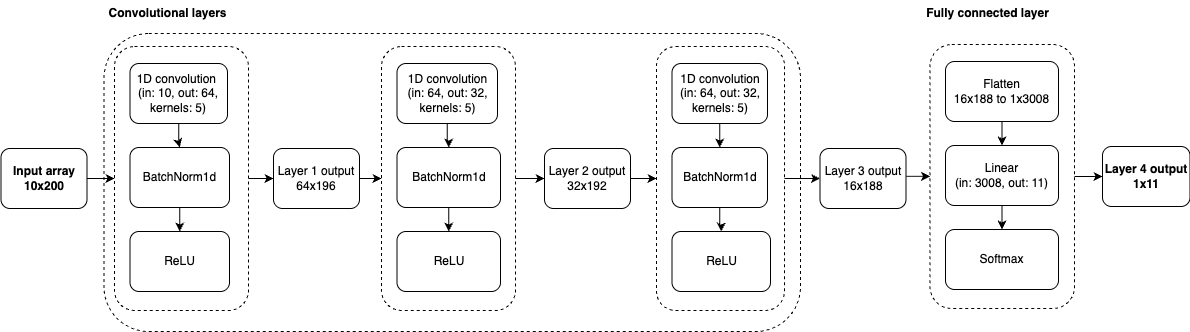
\includegraphics[width=\textwidth]{cnn-architecture-diagram.png}
    \caption{Diagram of the CNN architecture used in this study. It consists of three sequential 1D convolutional layers followed by batch normalization and ReLU activations, ending with a fully connected (FC) layer mapping to 11 gesture classes.}
    \label{image:cnn-architecture}
\end{figure*}
\begin{multicols}{2}

\subsection*{CNN Architecture}

The CNN architecture used in this study is based on implementations from works~\cite{Cote2019_3DC,LibEMG2023} and presented in the Fig.~\ref{image:cnn-architecture}. 
The network was designed to process raw surface EMG input of shape $10 \times 200$ (channels × samples).
All layer weights were initialized using the Glorot (Xavier) uniform method, with biases set to zero. The network was trained using the Adam optimizer, starting with a learning rate of $10^{-3}$, and a cosine annealing schedule was applied for learning rate adjustment. Cross-entropy was used as the loss function during training. Early stopping was applied with a patience of four epochs and tolerance threshold of 0.03. A maximum of 50 epochs was allowed during training, although convergence typically occurred within 15 epochs. To ensure reproducibility, all random seeds were explicitly set for PyTorch, NumPy, and Python’s built-in generators.
The exact implementation of the CNN used in this study is available in the publicly accessible repository~\cite{Kolomiiets2025}.

\subsection*{Evaluated training approaches}

All experiments in this study followed the same cross-validation protocol to ensure fair comparison. Specifically, a leave-one-out cross-validation (LOO-CV) strategy was applied to the repetitions of gesture sequences per subject. In each fold, one repetition was chosen for testing, one for validation during training, and the remaining ones for model training.

Three training approaches were explored. The first, referred to as \textit{Intra-subject training}, involved training and testing the model using data from the same individual. Different repetitions were used for training, validation, and testing, following the LOO-CV protocol.

The second approach, called \textit{Inter-subject training}, involved training the model on data from 21 participants and evaluating its performance on the one subject excluded from training. The same repetition-based LOO-CV was applied to each subject's data.

The third approach is named \textit{Transfer learning}, where a model pre-trained on the 21 training subjects was fine-tuned on data of the left-out subject. The same cross-validation setup described earlier was used here as well. Two fine-tuning strategies were investigated: one in which the fully connected (FC) output layer was reset before fine-tuning—referred to as \textit{Fine-tuning with FC reset}—and another where the FC layer remained unchanged, called \textit{Fine-tuning without FC reset}. In both cases, the convolutional layers of the model remained trainable during fine-tuning.

To further examine whether transfer learning with FC reset continues to perform better than training from scratch when subject-specific data is limited, additional experiments were conducted using fewer training repetitions. Instead of using all eight available repetitions, these used six, four, and three repetitions only. The same LOO-CV protocol was applied in each case to be consistent.

When all eight repetitions were used, the cross-validation process generated 56 folds per subject ($8 \times 7 = 56$), resulting in a total of 1232 folds across 22 subjects. With six repetitions, 30 folds per subject ($6 \times 5 = 30$) were produced, totaling 660 folds. For four repetitions, 12 folds per subject ($4 \times 3 = 12$) yielded 264 folds overall. Finally, for three repetitions, six folds per subject ($3 \times 2 = 6$) gave 132 folds in total.

The F1-score was used as the primary metric to evaluate classification accuracy. To determine whether the observed differences in performance were statistically significant, Wilcoxon signed-rank tests were applied to the distributions of F1-scores obtained from folds of each experiment.

\section{Results and discussion}


\subsection*{Compare training approaches}

Fig.~\ref{fig:boxplot-approaches} presents box-and-whisker plots summarizing the F1-score distributions for inter-subject generalization, intra-subject training, and two transfer learning strategies: fine-tuning with and without resetting the fully connected (FC) layer. All eight available repetitions were used for training in those experiments. Consequently, distributions are based on $1232 (8*7*22)$ cross-validation folds per training approach across all 22 subjects.

The inter-subject approach yielded a mean F1-score of 0.382 ($\sigma = 0.149$), confirming that generalization across subjects is significantly limited due to variability in electrode placement and anatomical differences. In contrast, intra-subject training—where the model is trained and tested on data from the same participant—achieved a dramatically higher mean F1-score of 0.869 ($\sigma = 0.089$).

Fine-tuning pre-trained models using the ``without FC reset'' transfer learning strategy further improved performance to 0.896 ($\sigma = 0.071$). However, the best result was obtained using the ``with FC reset'' transfer learning strategy, achieving a mean of 0.907 ($\sigma = 0.074$), suggesting that resetting the CNN's head enables better adaptation to new subjects. Both transfer learning strategies outperformed intra-subject training approach, affirming the benefit of using pre-trained models.

\subsection*{Evaluate the effect of reduced subject-specific data}

To assess whether transfer learning allowes to reduce the amount of subject-specific data, we additionally performed experiments with decreased numbers of training repetitions (6, 4, 3). As shown in Fig.~\ref{fig:boxplot-reps}, the transfer learning approach with FC layer reset consistently achieves higher F1-scores across all scenarios. While reducing the number of training repetitions to three results in a noticeable decline in accuracy, using four repetitions yields only a modest decrease. This effectively halves the required subject effort compared to using all eight repetitions, without substantially compromising classification accuracy.

\end{multicols}

\begin{figure*}[t]
\centering%{l}{\linewidth}
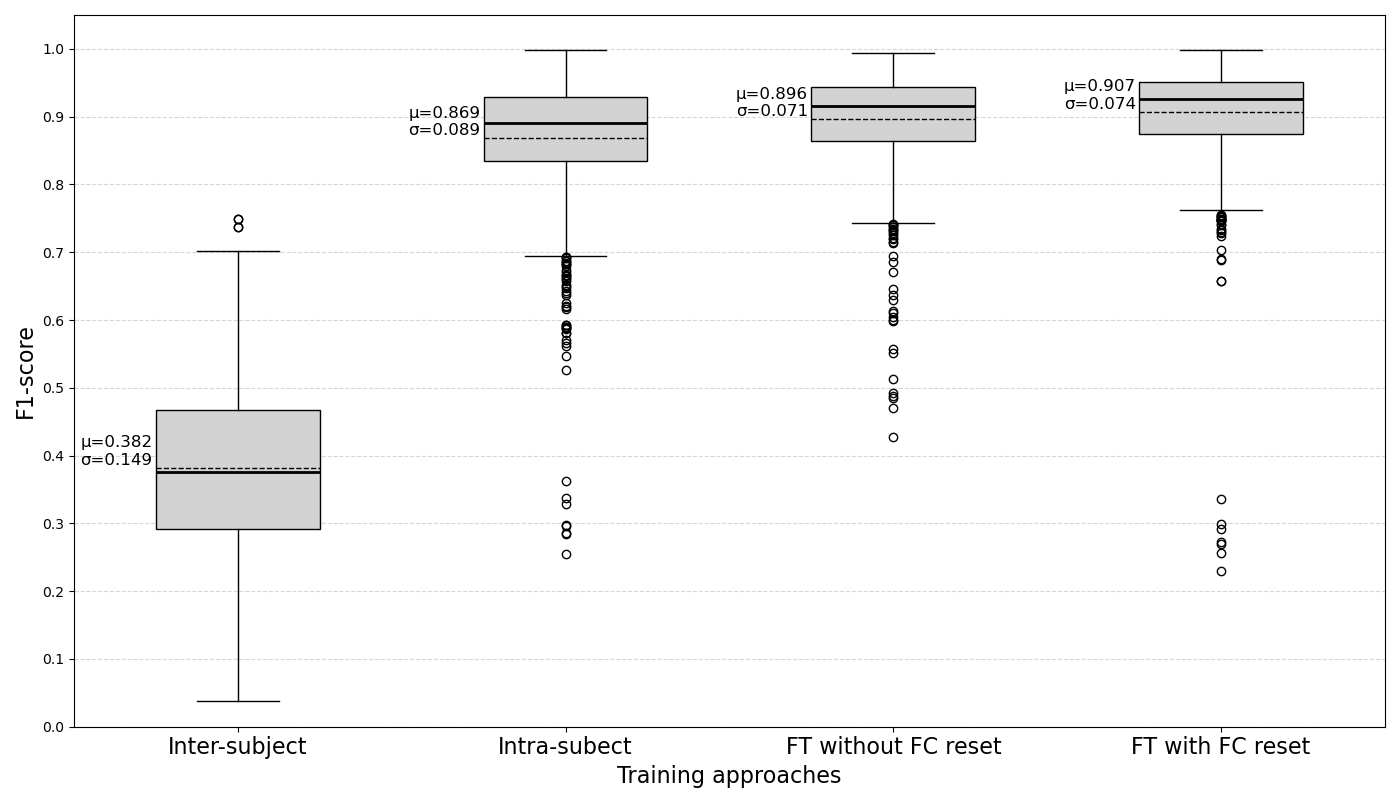
\includegraphics[width=\linewidth]{accuracy_by_approach_8_reps}
\captionof{figure}{Box-and-whisker plots of F1-score distributions across training approaches: ''Inter-subject', ''Intra-subject'' training approaches, and two fine-tuning (FT) strategies in transfer learning (TL) approach: with and without fully connected (FC) layer reset. Boxes represent interquartile range (IQR), lines show medians, and dashed lines indicate means. Outliers are shown as individual points.}
\label{fig:boxplot-approaches}
\end{figure*}

\begin{center}
\centering%{l}{\linewidth}
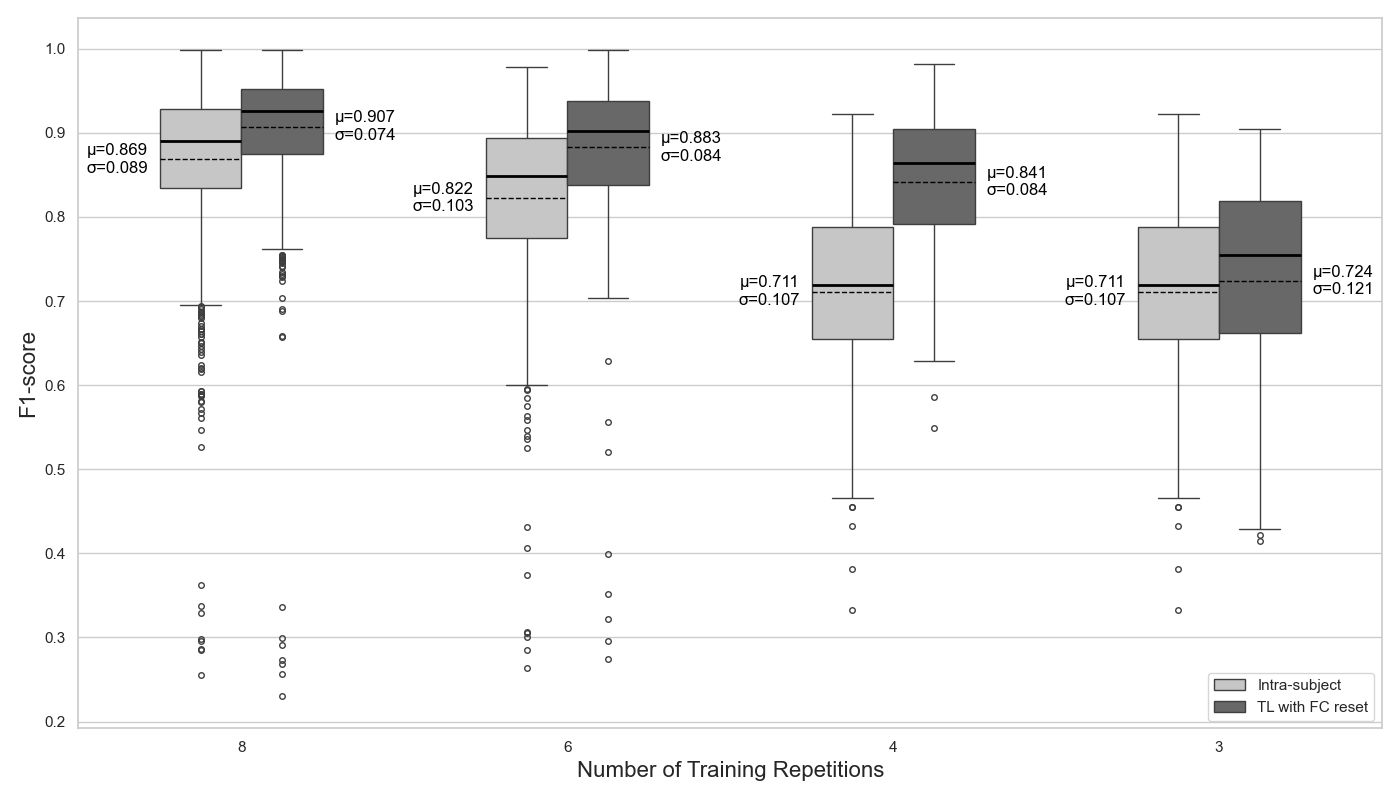
\includegraphics[width=\linewidth]{intra_subject_vs_fine_tuned_by_reps}
\captionof{figure}{Box-and-whisker plots showing the distribution of F1-scores across different numbers of training repetitions (6, 4, 2, 1) for ''Intra-subject'' and ''Transfer learning'' (TL) approach with fully connected (FC) layer reset. Note that repetitions numbers here represent a total number of repetitions consisting of eleven gestures a subject would need to execute to achieve shown accuracy. Each box shows the interquartile range and median; dashed lines denote the mean. Outliers are plotted as individual points.}
\label{fig:boxplot-reps}
\end{center}

\begin{table}[t]
\captionof{table}{Wilcoxon signed-rank test results comparing subject-wise F1-score means ($\mu$) and standard deviations ($\sigma$) across training strategies and training set sizes. $H_0$ represents null hypothesis, while $H_1$ - alternative hypothesis. TL+FC: Transfer Learning with FC reset; TL–FC: Transfer Learning without FC reset; Intra: Intra-subject training. The number of training repetitions used in each experiment is denoted by $r$. Bold horizontal lines separate hypothesis groups. Statistically significant results ($p < 0.05$) indicate a meaningful difference in accuracy or model stability.}
\begin{tabularx}{\linewidth}{|X|l|}
  \Xhline{2\arrayrulewidth}
  \textbf{Hypothesis} & \textbf{p-value} \\
  \Xhline{1\arrayrulewidth}
  \( H_0: \mu\left(\text{F1}_{\mathsf{TL{-}FC},\, r=8}\right) = \mu\left(\text{F1}_{\mathsf{Intra},\, r=8}\right) \) \newline
  \( H_1: \mu\left(\text{F1}_{\mathsf{TL{-}FC},\, r=8}\right) > \mu\left(\text{F1}_{\mathsf{Intra},\, r=8}\right) \)
  & $p = 7.87 \times 10^{-6} < 0.05$ \\
  \hline
  \( H_0: \sigma\left(\text{F1}_{\mathsf{TL{-}FC},\, r=8}\right) = \sigma\left(\text{F1}_{\mathsf{Intra},\, r=8}\right) \) \newline
  \( H_1: \sigma\left(\text{F1}_{\mathsf{TL{-}FC},\, r=8}\right) < \sigma\left(\text{F1}_{\mathsf{Intra},\, r=8}\right) \)
  & $p = 0.0829 > 0.05$ \\
  \Xhline{1.8\arrayrulewidth}
  \( H_0: \mu\left(\text{F1}_{\mathsf{TL{+}FC},\, r=8}\right) = \mu\left(\text{F1}_{\mathsf{Intra},\, r=8}\right) \) \newline
  \( H_1: \mu\left(\text{F1}_{\mathsf{TL{+}FC},\, r=8}\right) > \mu\left(\text{F1}_{\mathsf{Intra},\, r=8}\right) \)
  & $p = 2.38 \times 10^{-7} < 0.05$ \\
  \hline
  \( H_0: \sigma\left(\text{F1}_{\mathsf{TL{+}FC},\, r=8}\right) = \sigma\left(\text{F1}_{\mathsf{Intra},\, r=8}\right) \) \newline
  \( H_1: \sigma\left(\text{F1}_{\mathsf{TL{+}FC},\, r=8}\right) < \sigma\left(\text{F1}_{\mathsf{Intra},\, r=8}\right) \)
  & $p = 0.0016 < 0.05$ \\
  \Xhline{1.8\arrayrulewidth}
  \( H_0: \mu\left(\text{F1}_{\mathsf{TL{+}FC},\, r=8}\right) = \mu\left(\text{F1}_{\mathsf{TL{-}FC},\, r=8}\right) \) \newline
  \( H_1: \mu\left(\text{F1}_{\mathsf{TL{+}FC},\, r=8}\right) > \mu\left(\text{F1}_{\mathsf{TL{-}FC},\, r=8}\right) \)
  & $p = 3.46 \times 10^{-4} < 0.05$ \\
  \hline
  \( H_0: \sigma\left(\text{F1}_{\mathsf{TL{+}FC},\, r=8}\right) = \sigma\left(\text{F1}_{\mathsf{TL{-}FC},\, r=8}\right) \) \newline
  \( H_1: \sigma\left(\text{F1}_{\mathsf{TL{+}FC},\, r=8}\right) < \sigma\left(\text{F1}_{\mathsf{TL{-}FC},\, r=8}\right) \)
  &  $p = 0.118 > 0.05$ \\
  \Xhline{1.8\arrayrulewidth}
  \( H_0: \mu\left(\text{F1}_{\mathsf{TL{+}FC},\, r=6}\right) = \mu\left(\text{F1}_{\mathsf{Intra},\, r=6}\right) \) \newline
  \( H_1: \mu\left(\text{F1}_{\mathsf{TL{+}FC},\, r=6}\right) > \mu\left(\text{F1}_{\mathsf{Intra},\, r=6}\right) \)
  & $p = 2 \times 10^{-5} < 0.05$ \\
  \hline
  \( H_0: \sigma\left(\text{F1}_{\mathsf{TL{+}FC},\, r=6}\right) = \sigma\left(\text{F1}_{\mathsf{Intra},\, r=6}\right) \) \newline
  \( H_1: \sigma\left(\text{F1}_{\mathsf{TL{+}FC},\, r=6}\right) < \sigma\left(\text{F1}_{\mathsf{Intra},\, r=6}\right) \)
  & $p = 0.033 < 0.05$ \\
  \Xhline{1.8\arrayrulewidth}
  \( H_0: \mu\left(\text{F1}_{\mathsf{TL{+}FC},\, r=4}\right) = \mu\left(\text{F1}_{\mathsf{Intra},\, r=4}\right) \) \newline
  \( H_1: \mu\left(\text{F1}_{\mathsf{TL{+}FC},\, r=4}\right) > \mu\left(\text{F1}_{\mathsf{Intra},\, r=4}\right) \)
  & $p = 2 \times 10^{-5} < 0.05$ \\
  \hline
  \( H_0: \sigma\left(\text{F1}_{\mathsf{TL{+}FC},\, r=4}\right) = \sigma\left(\text{F1}_{\mathsf{Intra},\, r=4}\right) \) \newline
  \( H_1: \sigma\left(\text{F1}_{\mathsf{TL{+}FC},\, r=4}\right) < \sigma\left(\text{F1}_{\mathsf{Intra},\, r=4}\right) \)
  & $p = 0.0018 < 0.05$ \\
  \Xhline{1.8\arrayrulewidth}
  \( H_0: \mu\left(\text{F1}_{\mathsf{TL{+}FC},\, r=3}\right) = \mu\left(\text{F1}_{\mathsf{Intra},\, r=3}\right) \) \newline
  \( H_1: \mu\left(\text{F1}_{\mathsf{TL{+}FC},\, r=3}\right) > \mu\left(\text{F1}_{\mathsf{Intra},\, r=3}\right) \)
  & $p = 2 \times 10^{-5} < 0.05$ \\
  \hline
  \( H_0: \sigma\left(\text{F1}_{\mathsf{TL{+}FC},\, r=3}\right) = \sigma\left(\text{F1}_{\mathsf{Intra},\, r=3}\right) \) \newline
  \( H_1: \sigma\left(\text{F1}_{\mathsf{TL{+}FC},\, r=3}\right) < \sigma\left(\text{F1}_{\mathsf{Intra},\, r=3}\right) \)
  & $p = 0.0473 < 0.05$ \\
  \Xhline{2\arrayrulewidth}
\end{tabularx}
\label{table:statistical-tests}
\end{table}

\begin{multicols}{2}

\subsection*{Statistical significance of transfer learning improvements}

To assess whether the observed differences in model performance were statistically meaningful, Wilcoxon signed-rank tests were applied to compare subject-wise F1-score means ($\mu$) and standard deviations ($\sigma$). Table~\ref{table:statistical-tests} summarizes the results for all training approaches and repetition settings evaluated in this study.

When all eight repetitions were used for training, transfer learning without FC reset showed a statistically significant improvement in mean F1-score over intra-subject training ($p = 7.87 \times 10^{-6}$), though its gain in model stability was not significant ($p = 0.0829$). In contrast, transfer learning with FC reset demonstrated both a significant increase in classification accuracy ($p = 2.38 \times 10^{-7}$), as well as a significant reduction in F1-score variability ($p = 0.0016$), indicating improved consistency across cross-validation folds. Furthermore, direct comparison of the two transfer learning strategies showed that resetting the FC layer led to significantly higher mean F1-scores ($p = 3.46 \times 10^{-4}$), though the difference in standard deviations remained statistically insignificant ($p = 0.118$).

The advantage of fine-tuning with FC reset remained consistent across all tested repetition counts. When training data was reduced to six, four, or even three repetitions, the mean F1-score remained significantly higher compared to intra-subject models trained under the same constraints. In each of these scenarios, Wilcoxon tests confirmed not only higher accuracy but also significantly lower variability in model performance (all $p < 0.05$), even under data-limited conditions.

The results of all training experiments, as well as the Python scripts used for statistical evaluation, are available in the publicly accessible repository~\cite{Kolomiiets2025}.

Overall, thse findings confirm that transfer learning strategies offer statistically robust improvements in terms of gesture classification accuracy. Among the evaluated strategies, fine-tuning with FC reset provides statistically better accuracy and stability, regardless of how much subject-specific data is available. The ability to retain these advantages under reduced-data conditions supports its suitability for real-world deployment, especially in real-time or wearable applications where minimizing calibration effort is essential.

\subsection*{Limitations, Comparison to Related Work, and Future Directions}

While our experiments clearly show that transfer learning improves model accuracy and stability, there are some limitations to consider.

First, the CNN model we used is relatively simple. We chose this to keep training fast and make our results easier to compare with past research~\cite{Cote2019_3DC,LibEMG2023}. However, more advanced models like temporal convolutional networks~\cite{Xie2024} or CNN–LSTM combinations~\cite{Faust2018} may be able to improve accuracy further.

Second, the 3DC dataset was designed to simulate real-world changes in electrode placement, which is good for testing generalization. But this also adds noise to the data, which may lower accuracy compared to more controlled datasets.

Third, all experiments were done offline. To test if the models work in real-world use, future studies should evaluate performance in real-time conditions, such as wearable systems or interactive applications~\cite{Shen2020}.

Compared to earlier works like Côté-Allard et al.~\cite{Cote2019}, which showed the benefits of transfer learning for sEMG, our study goes further by comparing two fine-tuning strategies and measuring their statistical significance. Other studies~\cite{Lehmler2021, Ameri2020} looked at transfer learning across electrode shifts, but few have measured how much subject-specific data can be saved. This is a key contribution of our work.

In the future, it would be useful to test more complex models, add domain adaptation techniques, and use fewer labeled samples. Testing the models on small devices like microcontrollers would also show how well they work in real applications. Public benchmarks on larger and more varied datasets would also help to confirm how well these results generalize. The source code and evaluation results for this study available publicly~\cite{Kolomiiets2025} can help other researchers build on this work.

\section*{Conclusion}

This study investigated the effectiveness of transfer learning for surface electromyography (sEMG) gesture classification using convolutional neural network (CNN). By comparing intra-subject training, inter-subject generalization, and two transfer learning strategies (with and without resetting the FC layer), we demonstrated that transfer learning significantly enhances classification performance and model stability.

Our experiments showed that fine-tuning pre-trained models—especially when resetting the FC layer—not only improves F1-scores but also reduces standard deviation across cross-validation folds, indicating more consistent performance. Notably, this benefit remains statistically significant even when using a reduced number of repetitions for subject-specific fine-tuning, suggesting that transfer learning can substantially reduce the effort required for user calibration.

In addition, the statistical analysis using Wilcoxon signed-rank tests confirmed the superiority of the fine-tuned models under various data constraints. These findings emphasize the practicality of transfer learning in real-world applications where data availability is limited.

Nevertheless, the study has several limitations. The CNN architecture used is relatively simple and may not capture more complex spatiotemporal dependencies in the EMG signal. Also, evaluations were conducted in an offline setting using a single dataset (3DC), which, while realistic in variability, may not generalize to all EMG acquisition systems or environments.

Future works could explore deeper and hybrid models, real-time implementations, and domain adaptation techniques to further reduce calibration overhead. Expanding evaluation to diverse datasets and hardware platforms will be critical to validating these results at scale.

In summary, transfer learning—particularly fine-tuning with FC reset—showed itself as an effective strategy for subject adaptation in sEMG-based gesture recognition, offering performance and stability improvements, as well as reducing amount of training data needed.

\pdfbookmark[1]{References}{translit}
\renewcommand{\refname}{References}

\begin{thebibliography}{99}\footnotesize 

\bibitem{Zhou2023}
Zhou, Y., Wang, Y., Wang, X., \& Zhang, Y., 2023. Electromyography monitoring systems in rehabilitation: A review of current applications and future challenges. \textit{Electronics}, 12(7), p.1520. Available at: \url{https://doi.org/10.3390/electronics12071520} [Accessed 25 May 2025].

\bibitem{Xie2024}
Xie, P., Xu, M., Shen, T., Chen, J., Jiang, G., Xiao, J., \& Chen, X., 2024. A channel-fused gated temporal convolutional network for EMG-based gesture recognition. \textit{Biomedical Signal Processing and Control}, 95, 106408. Available at: \url{https://doi.org/10.1016/j.bspc.2024.106408} [Accessed 25 May 2025].

\bibitem{Merletti2020}
Merletti, R. \& Farina, D., 2020. Tutorial. Surface EMG detection, conditioning and pre-processing: Best practices. \textit{Journal of Electromyography and Kinesiology}, 54, p.102440. Available at: \url{https://doi.org/10.1016/j.jelekin.2020.102440} [Accessed 25 May 2025].

\bibitem{Plux2022}
Plux Biosignals, 2022. Where should I place my Electromyography (EMG) electrodes? Available at: \url{https://support.pluxbiosignals.com/knowledge-base/where-should-i-place-my-electromyography-emg-electrodes/} [Accessed 25 May 2025].

\bibitem{Chowdhury2013}
Chowdhury, R.H., Reaz, M.B.I., Ali, M.A.B.M., Bakar, A.A.A., Chellappan, K., \& Chang, T.G., 2013. Surface electromyography signal processing and classification techniques. \textit{Sensors}, 13(9), pp.12431–12466. Available at: \url{https://doi.org/10.3390/s130912431} [Accessed 25 May 2025].

\bibitem{Phinyomark2019}
Phinyomark, A., Campbell, E., \& Scheme, E., 2019. Surface electromyography (EMG) signal processing, classification, and practical considerations. In: G. Naik, ed., \textit{Biomedical Signal Processing}. Singapore: Springer, pp.3–29. Available at: \url{https://doi.org/10.1007/978-981-13-9097-5_1} [Accessed 25 May 2025].

\bibitem{Faust2018}
Faust, O., Hagiwara, Y., Hong, T.J., Lih, O.S. \& Acharya, U.R., 2018. Deep learning for healthcare applications based on physiological signals: A review. \textit{Computer Methods and Programs in Biomedicine}, 161, pp.1–13. Available at: \url{https://doi.org/10.1016/j.cmpb.2018.04.005} [Accessed 25 May 2025].

\bibitem{Wu2022}
Wu, D., Yang, J., \& Sawan, M., 2022. Transfer learning on electromyography (EMG) tasks: Approaches and beyond. \textit{arXiv preprint arXiv:2210.06295}. Available at: \url{https://arxiv.org/abs/2210.06295} [Accessed 25 May 2025].

\bibitem{Cote2019}
Côté-Allard, U., Fall, C.L., Campeau-Lecours, A., et al., 2019. Deep learning for electromyographic hand gesture signal classification using transfer learning. \textit{IEEE Transactions on Neural Systems and Rehabilitation Engineering}, 27(4), pp.760–771. Available at: \url{https://doi.org/10.1109/TNSRE.2019.2896269} [Accessed 25 May 2025].

\bibitem{Ameri2020}
Ameri, A., Akhaee, M.A., Scheme, E. \& Englehart, K.B., 2020. A deep transfer learning approach to reducing the effect of electrode shift in EMG pattern recognition-based control. \textit{IEEE Transactions on Neural Systems and Rehabilitation Engineering}, 28(2), pp.370–379. Available at: \url{https://doi.org/10.1109/TNSRE.2019.2962189} [Accessed 25 May 2025].

\bibitem{Shen2020}
Shen, S., Gu, K., Chen, X.-R., Lv, C.-X., \& Wang, R.-C., 2020. Gesture recognition through sEMG with wearable device based on deep learning. \textit{Mobile Networks and Applications}, 25(6), pp.2447–2458. Available at: \url{https://doi.org/10.1007/s11036-020-01590-8} [Accessed 25 May 2025].

\bibitem{Geng2016}
Geng, Y., Zhou, P. \& Li, G., 2016. Toward attenuating the impact of inter-session variability in myoelectric pattern recognition using adaptive sparse representation. \textit{Journal of NeuroEngineering and Rehabilitation}, 13(1), p.4. Available at: \url{https://doi.org/10.1186/s12984-015-0114-3} [Accessed 25 May 2025].

\bibitem{Lehmler2021}
Lehmler, S.J., Saif-ur-Rehman, M., Glasmachers, T. \& Iossifidis, I., 2021. Deep transfer-learning for patient specific model re-calibration: Application to sEMG-classification. \textit{arXiv preprint arXiv:2112.15019}. Available at: \url{https://arxiv.org/abs/2112.15019} [Accessed 25 May 2025].

\bibitem{Cote2019_3DC}
Côté-Allard, U., Campbell, E., Phinyomark, A., et al., 2019. A low-cost, wireless, 3D-printed custom armband for sEMG hand gesture recognition. \textit{Sensors}, 19(12), 2811. Available at: \url{https://doi.org/10.3390/s19122811} [Accessed 25 May 2025].

% Methods
\bibitem{LibEMG2023}
Campeau-Lecours, A., Bouchard, D., Côté-Allard, U. and Gosselin, B., 2023. LibEMG: An Open Source Library to Facilitate the Exploration of Myoelectric Control. \textit{IEEE Access}, 11, pp.88686–88702. Available at: \url{https://doi.org/10.1109/ACCESS.2023.3304544} [Accessed 25 May 2025].

\bibitem{Smith2011}
Smith, L.H., Hargrove, L.J., Lock, B.A. and Kuiken, T.A., 2011. Determining the optimal window length for pattern recognition-based myoelectric control: balancing the competing effects of classification error and controller delay. \textit{IEEE Transactions on Neural Systems and Rehabilitation Engineering}, 19(2), pp.186--192. Available at: \url{https://doi.org/10.1109/TNSRE.2010.2100828} [Accessed 26 May 2025].

\bibitem{Rehman2018}
Rehman, M.Z.U., Waris, A., Gilani, S.O., Jochumsen, M., Niazi, I.K., Jamil, M., Farina, D. and Kamavuako, E.N., 2018. Multiday EMG-Based Classification of Hand Motions With Deep Learning Techniques. \textit{Sensors}, 18(8), p.2497. Available at: \url{https://doi.org/10.3390/s18082497} [Accessed 25 May 2025].

\bibitem{Oskoei2007}
Oskoei, M.A. and Hu, H., 2007. Myoelectric control systems—A survey. \textit{Biomedical Signal Processing and Control}, 2(4), pp.275–294. Available at: \url{https://doi.org/10.1016/j.bspc.2007.07.009} [Accessed 25 May 2025].

\bibitem{Kolomiiets2025}
Kolomiiets, B. Yu., 2025. *Code used for experiments presented in this artcile* [online]. GitHub. Available at: \url{https://github.com/bohdan-kolomiiets/phd-article-1} [Accessed 27 May 2025].

\end{thebibliography}